\section{测试}

\subsection{性能测试}

我们在监控程序中对所提供的5个流水线性能测试程序进行测试,得到的结果如\tref{table:per_test}所示。CPU主频为20MHz。

\begin{center}
    \tcaption{流水线性能测试结果}\label{table:per_test}
    \begin{longtable}{cccc}
        \toprule
        测试程序 & 运行时间 (s) & 指令条数 (亿) & CPI \\
        \midrule
        1 & 6.257 & 1.25 & 1.001 \\
        2 & 10.005 & 2.00 & 1.000 \\
        3 & 4.992 & 1.00 & 0.998 \\
        4 & 4.993 & 1.00 & 0.999 \\
        5 & 4.994 & 0.75 & 1.332 \\
        \bottomrule
    \end{longtable}
\end{center}

可见,除了读写指令内存需要插气泡,导致CPI增加以外,其他程序运行的CPI都接近于1,说明数据旁路对于冲突处理得很好,只有在少数情况下才需要暂停流水线。

\subsection{扩展指令测试}

我们编写了两段程序用于测试扩展指令的正确性。

\subsubsection{扩展指令测试程序1}

程序源码为

\lstset{basicstyle=\small\ttfamily, numbers=left}
\begin{lstlisting}
    LI R0 40
    SLL R0 R0 0
    ADDIU R0 0A
    LI R1 0
    LI R2 0
    LI R3 0
    LI R4 0
    JALR R0
    JR R7
    NOP
    NOT R1 R1
    NOT R2 R2
    NOT R3 R3
    NOT R4 R4
    JRRA
    NOP
\end{lstlisting}

这段程序的功能是:置R0至R4为0,然后通过JALR指令进行过程调用,跳转到0x400A,即这里的第10行,从而完成把R1至R4分别取反赋给它们自己,即变为0xFFFF。运行前后寄存器值如\fref{fig:testp1}所示,说明结果正确。

\begin{center}
    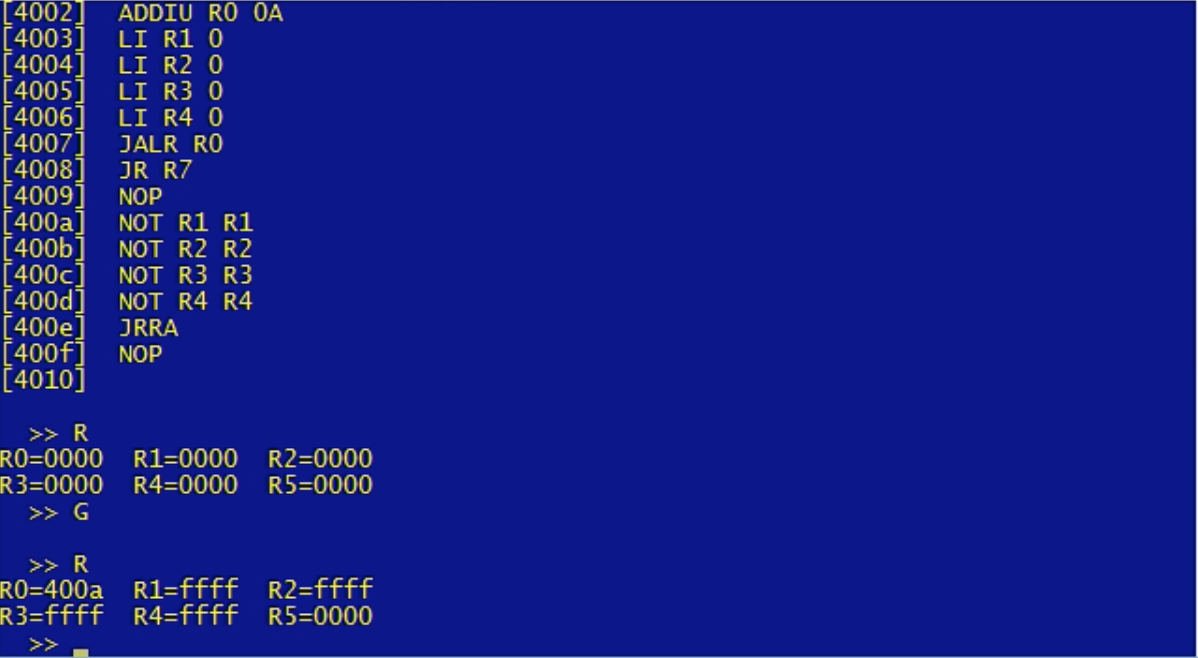
\includegraphics[width=13cm]{image/testing/p1}
    \fcaption{测试程序1运行结果}\label{fig:testp1}
\end{center}

这段程序验证了\texttt{NOT}, \texttt{JALR}, \texttt{JRRA}的正确性。

\subsubsection{扩展指令测试程序2}

程序源码为

\begin{lstlisting}
    LI R0 1
    LI R1 2
    SLT R0 R1
    BTNEZ 5
    NOP
    LI R3 80
    JR R7
    NOP
    LI R5 0
    NOT R5 R5
    SLT R1 R0
    BTNEZ FA
    NOP
    JR R7
    NOP
\end{lstlisting}

这段程序的功能是:置R0为1,置R1为2。第3行处由于R0<R1,置T为1。由于T不等于0,第4行的跳转会被执行。即从第9行开始执行,R5先被置0,然后取反,结果为0xFFFF。之后由于R1>R0,故第12行的跳转不会执行,直接退出用户程序,返回监控程序。假设第12行跳转执行,那么在第6行R3会被赋值为0x80。运行前后寄存器值如\fref{fig:testp2}所示,R3的值未改变,而R5变成0xFFFF,说明结果正确。

\begin{center}
    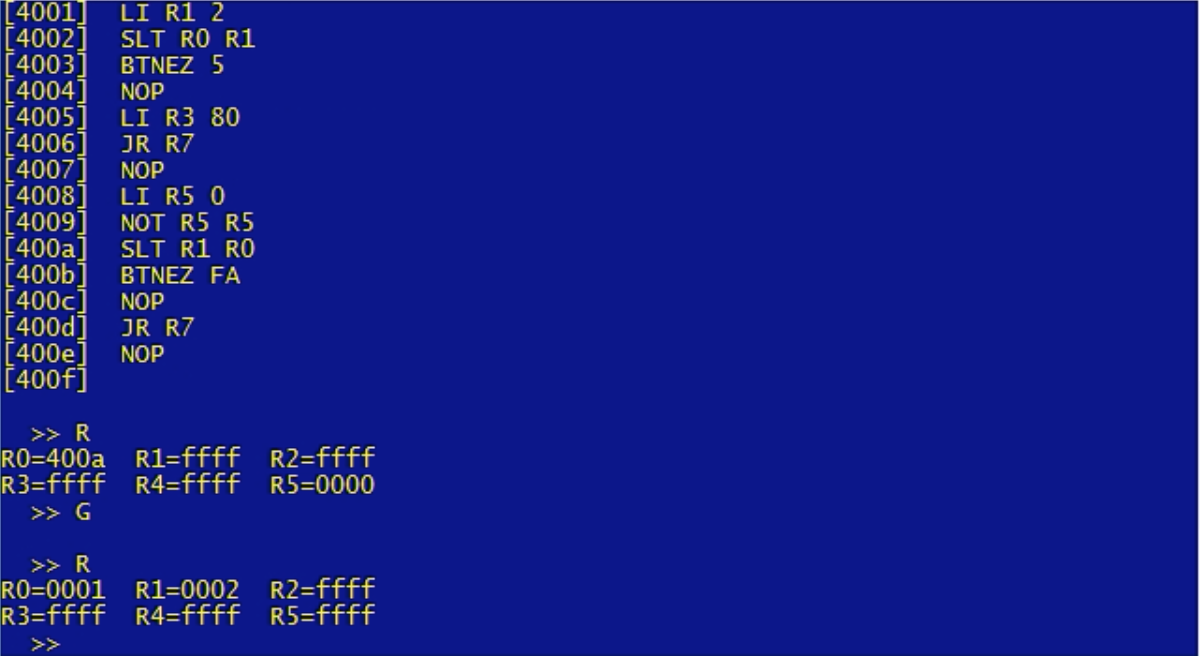
\includegraphics[width=13cm]{image/testing/p2}
    \fcaption{测试程序2运行结果}\label{fig:testp2}
\end{center}

这段程序验证了\texttt{SLT}, \texttt{BTNEZ}的正确性。

\subsection{外设与中断测试}

这部分我们采用了一个绘图程序用来展示VGA的像素映射功能与键盘输入功能。由于是硬件中断,我们可以发现在键盘输入后屏幕上会立即响应,同时已经绘制好的图形也不受影响。如\fref{fig:vga_keyboard}所示。

\begin{center}
    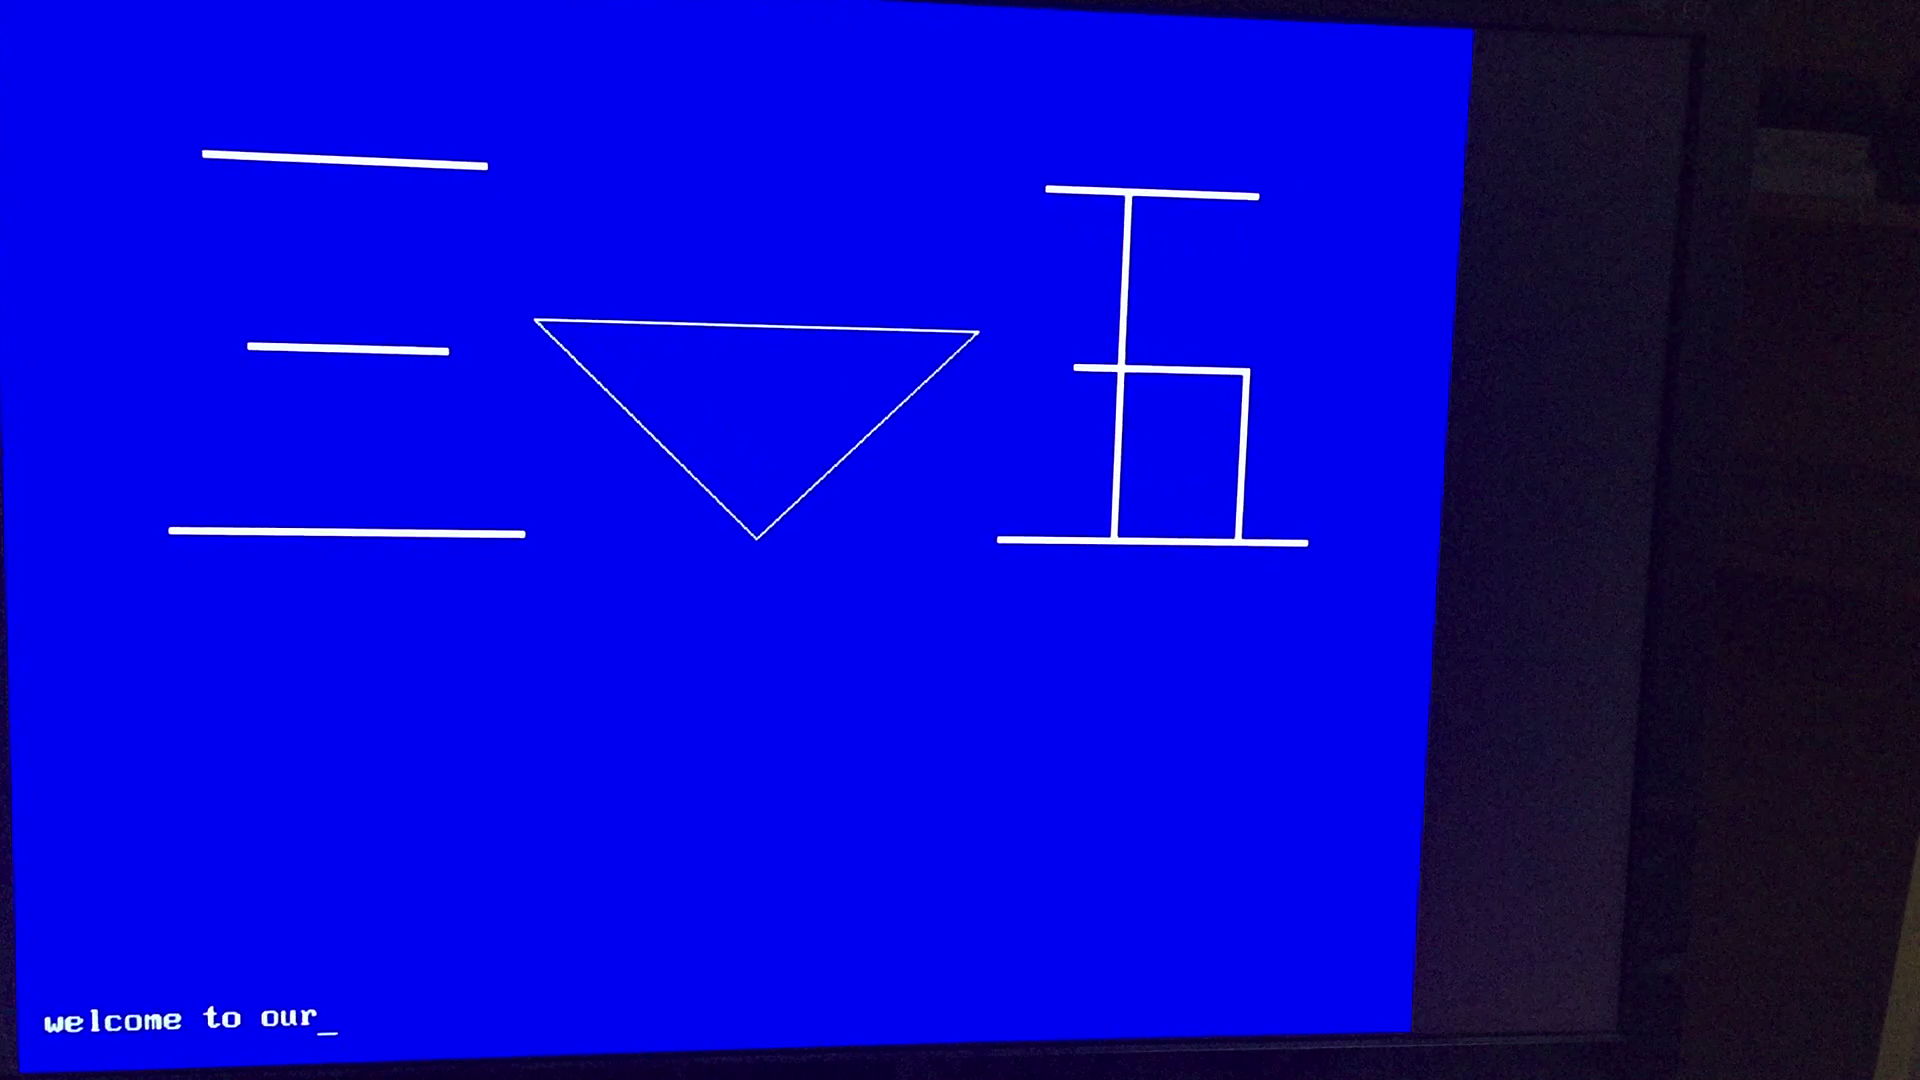
\includegraphics[width=13cm]{image/testing/vga_keyboard}
    \fcaption{外设演示}\label{fig:vga_keyboard}
\end{center}

键盘不仅可以输入,还可以按空格键清除输入的内容。

\begin{center}
    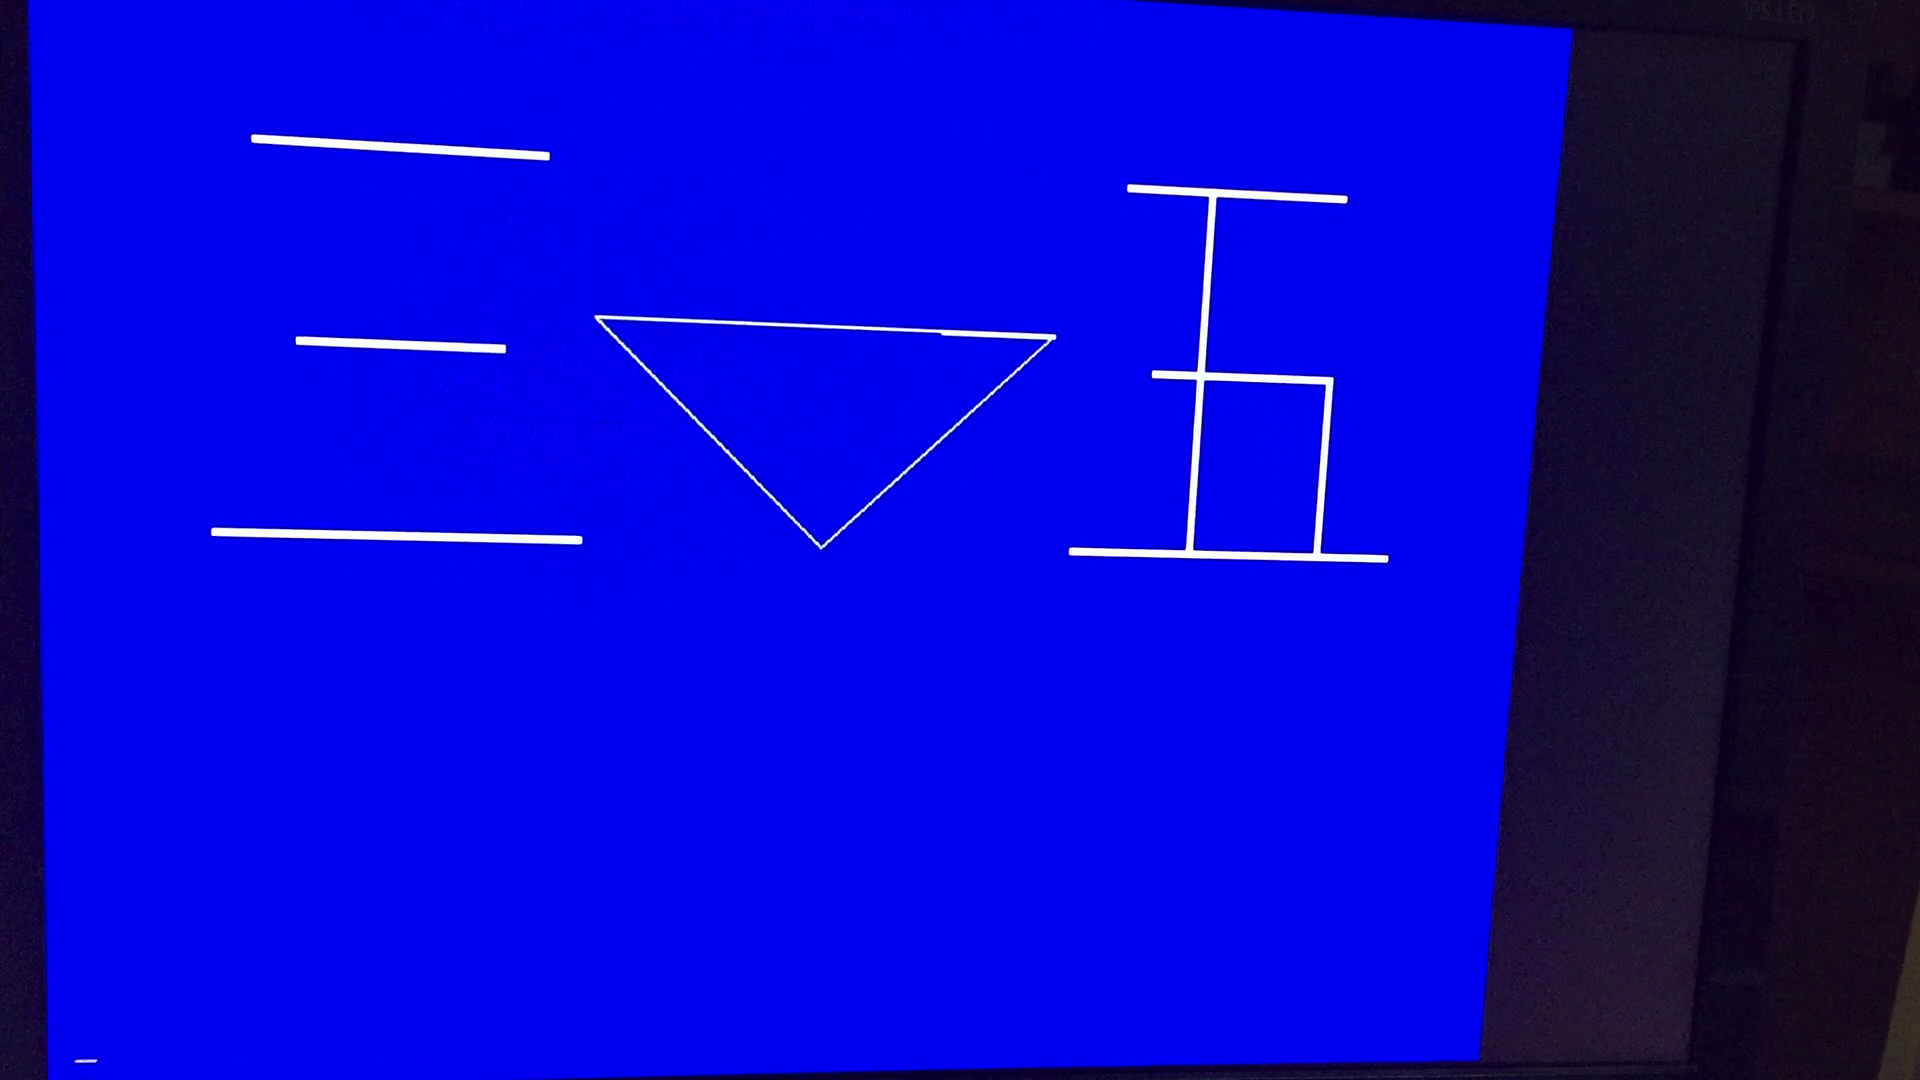
\includegraphics[width=13cm]{image/testing/clear}
    \fcaption{按空格键清屏}
\end{center}

此外,键盘还支持大小写输入。即,键盘不仅能捕获到单个键,还能捕获到组合键,如输入大写的A则在按下SHIFT键同时按下A。

\begin{center}
    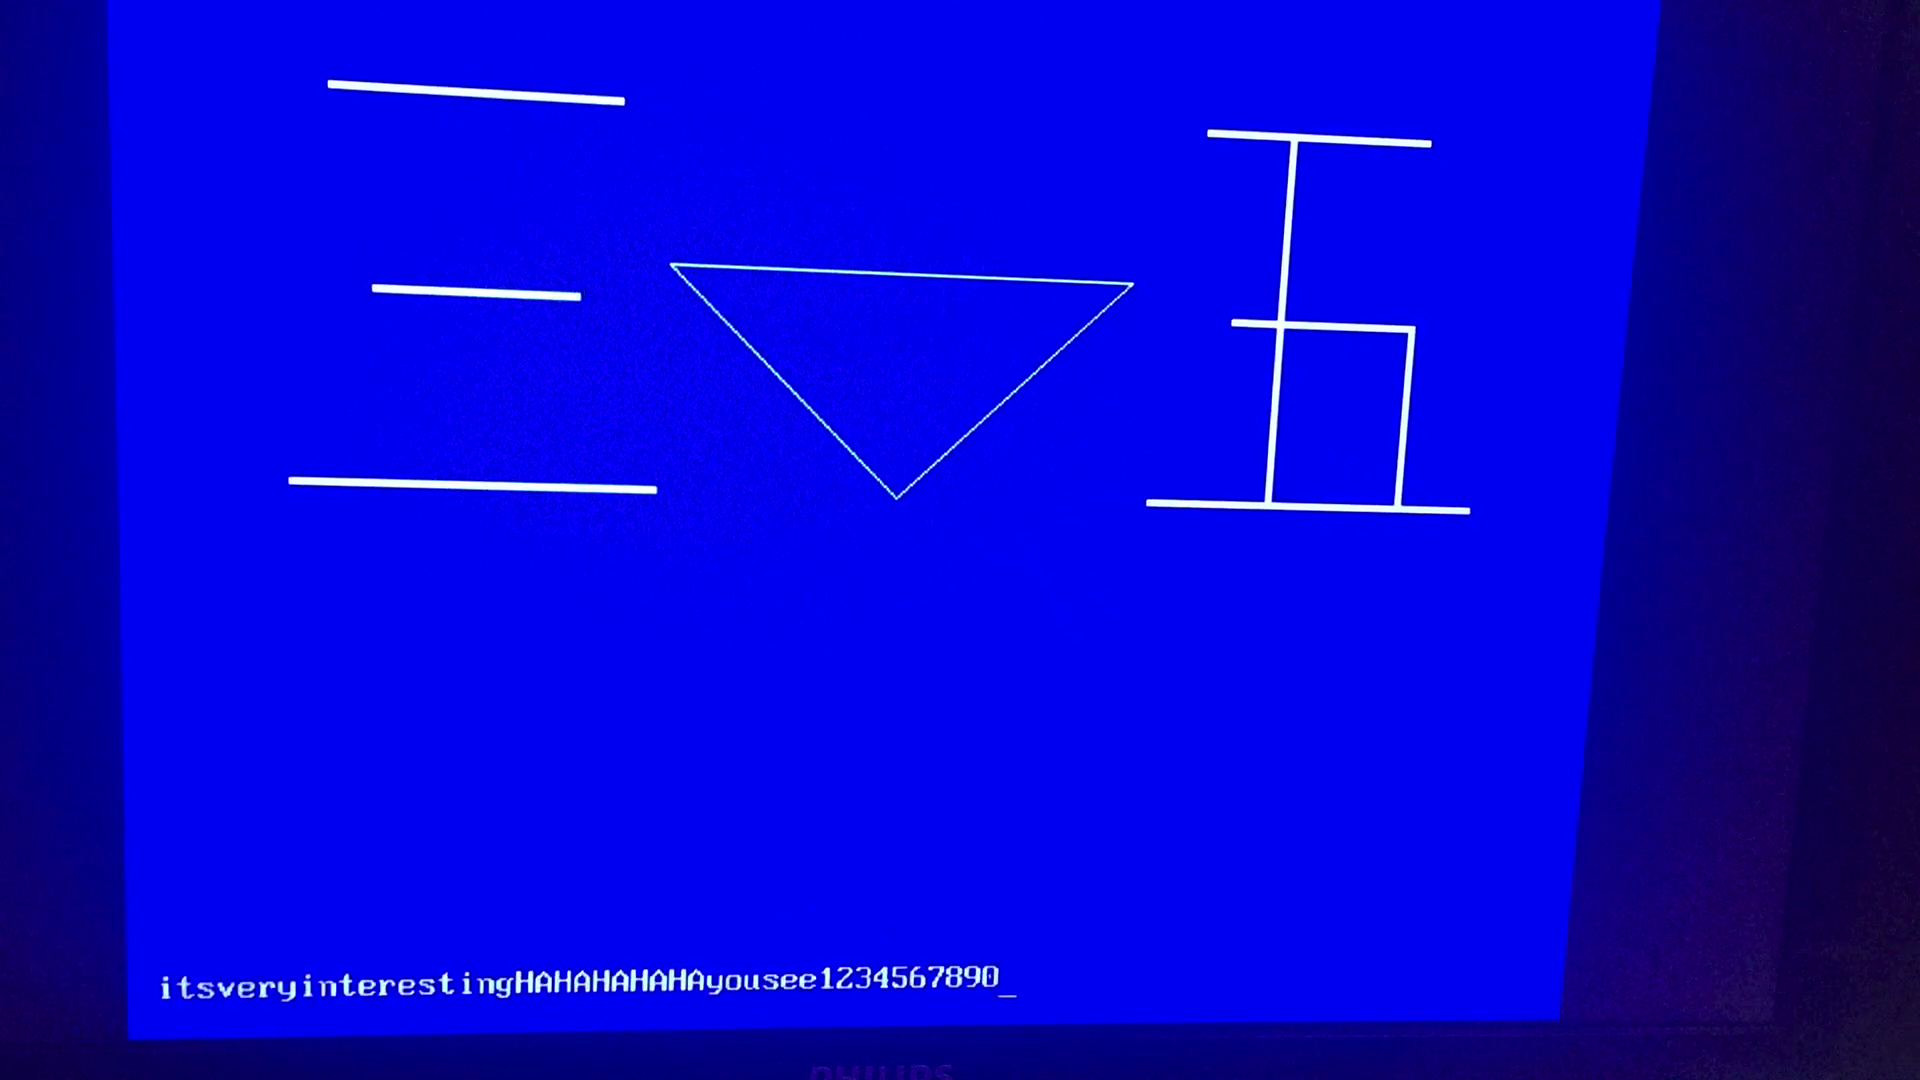
\includegraphics[width=13cm]{image/testing/case}
    \fcaption{大小写字符均可输入}
\end{center}

当输入错误时还可以按退格键删除一个字符。

\begin{center}
    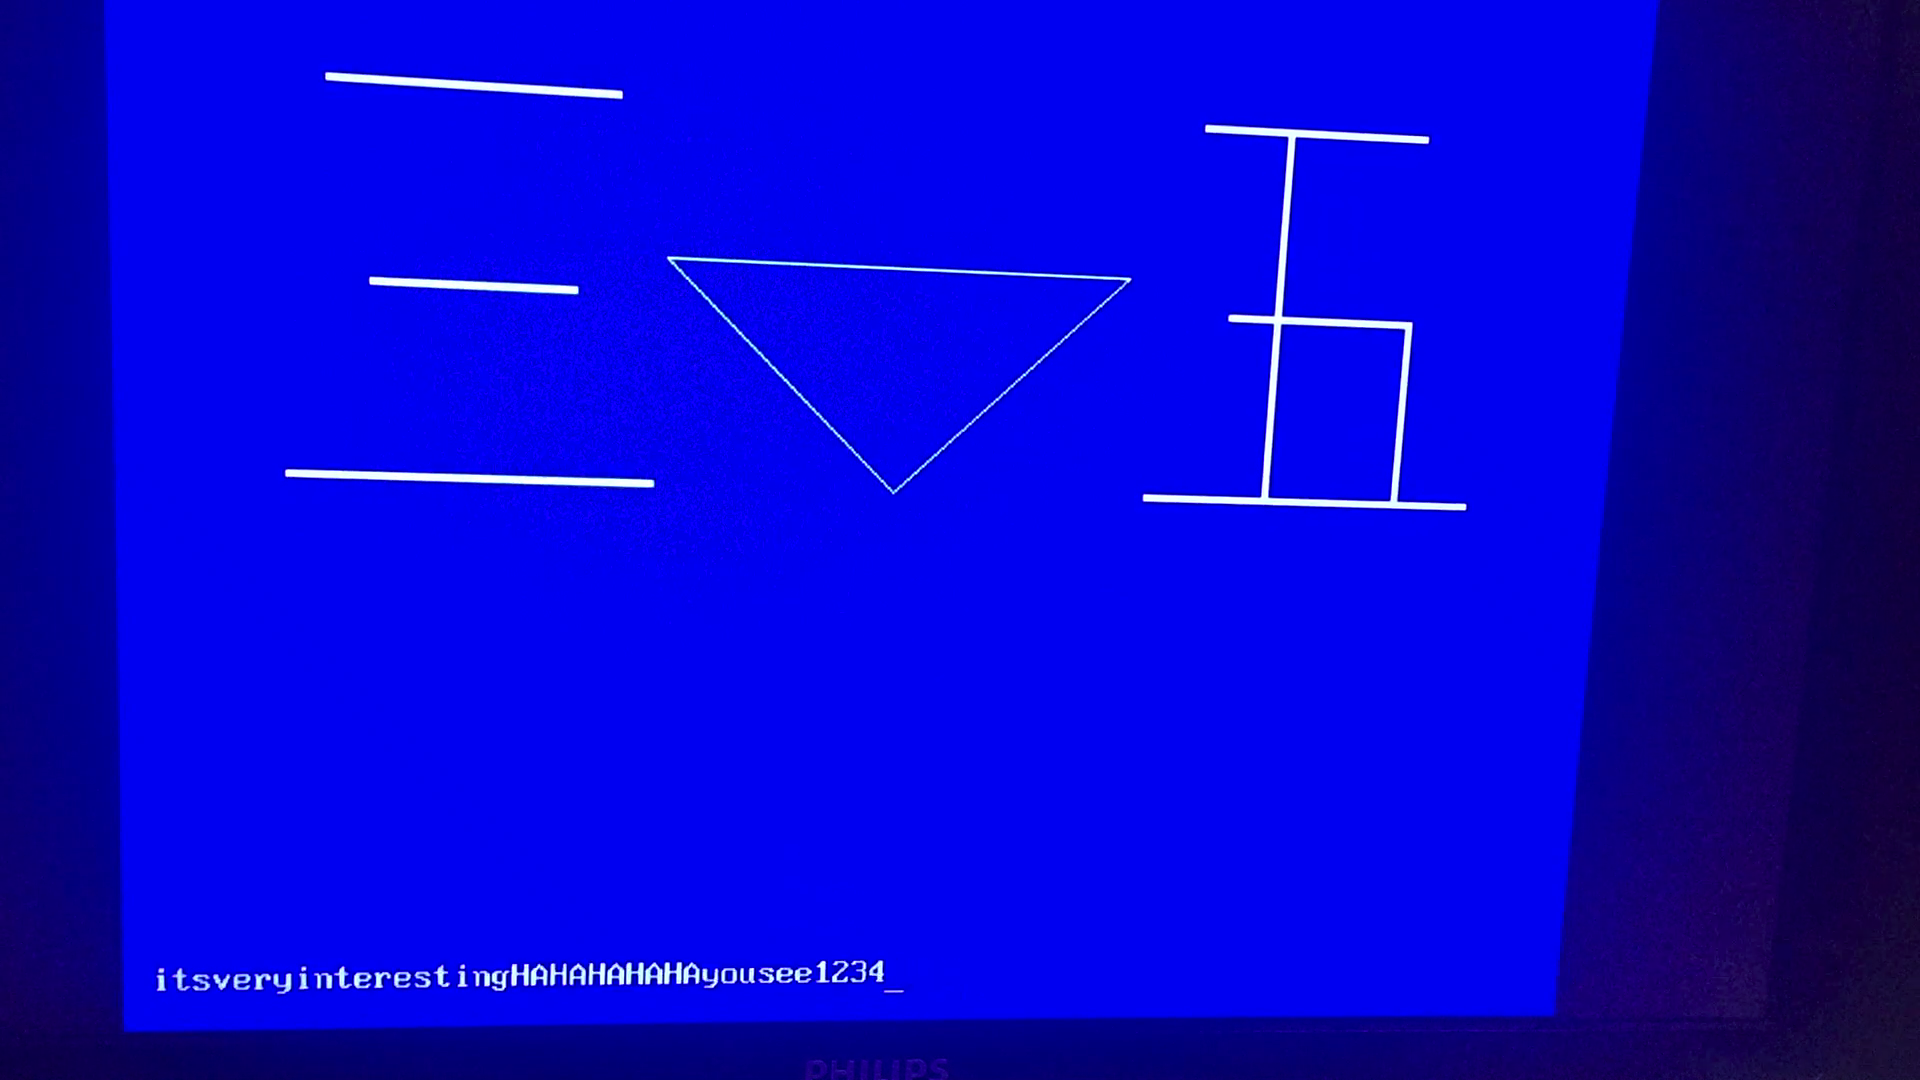
\includegraphics[width=13cm]{image/testing/backspace}
    \fcaption{退格}
\end{center}

至此,我们实现的所有30条指令以及自己扩展的\texttt{ERET}指令均通过了测试。
